\documentclass[../part_2.tex]{subfiles}

\begin{document}
    \subsection{Алгоритм обучения}
    \par Для обучения было решено модернизировать алгоритм dino для работы с текстом.
    \par Для этого было необходимо сделать
    \begin{itemize}
        \item Переработать модель из ViT в Transformer
        \item Преобразовать multicrop augmentation
        \item Выбрать подходящие аугментации
    \end{itemize}
    \subsubsection{Описание архитектуры самой маленькой нейронной сети из представленных}    
    \par Изначально архитектура разбивала исходное изображение на кусочки размером $16\times16$ пикселей, потом при помощи линейного преобразования преобразовывались в вектора embedding. Затем к ним прибавлялись Positional Embeddig и эти данные передавались дальше в блоки модели.
    \begin{figure}[H]
        \centering
        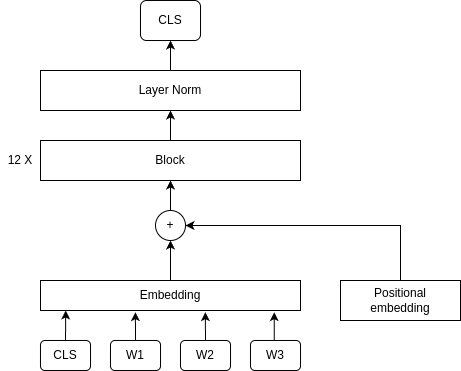
\includegraphics[width=0.6\textwidth]{model_arc.png}
        \caption{Архитектура нейросети}
        \label{fig:model_arc}
    \end{figure}
    \par Для изменения линейного преобразования был использован Embedding слой, который каждому токену присваивает свой вектор представления.
    \begin{figure}[H]
        \centering
        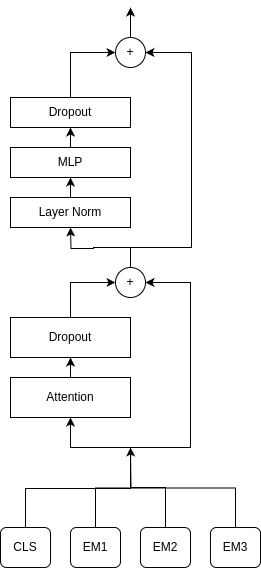
\includegraphics[height=0.6\textwidth]{nn_block.png}
        \caption{Архитектура блока нейросети}
        \label{fig:nn_block}
    \end{figure}
    \par Блок состоит из слоя нормирования, внимания, dropout, еще раз нормирования и MLP. Из них самым полезным и ресурсозатратным является слой внимания. Его вычисление зависит от квадрата числа токенов в последовательности.
    \par Так как изначальное изображение было размером $224\times224$, то в Vit модели было всего 196 токенов. В текстовой же реализации токенов значительно больше.
    \begin{figure}[H]
        \centering
        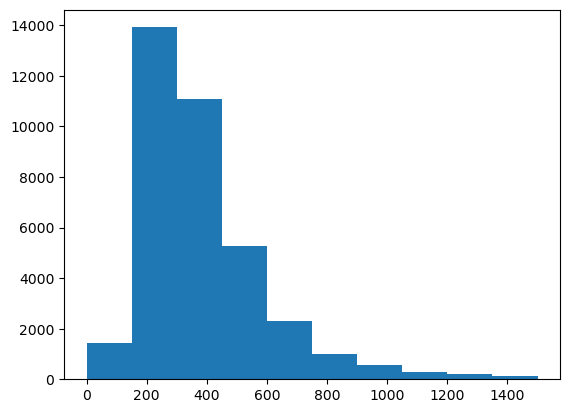
\includegraphics[width=0.6\textwidth]{tok_len_hist.png}
        \caption{Гистограмма распределения количества токенов в объектах тренировочного набора}
        \label{fig:tok_len_hist}
    \end{figure}
    \par Из рисунка \ref{fig:tok_len_hist} видно что оптимальным количеством токенов для рассмотрения будет 1000, что в 5 раз больше привычного количества токенов у блока. Соответственно вычисление attention становится медленнее в 25 раз.
    \par В связи с неэффективностью стандартного attention слоя, было решено использовать встроенный в PyTorch FalshAttention\cite{dao2022flashattentionfastmemoryefficientexact}. Таким образом удалось существенно увеличить скорость работы и уменьшить потребление памяти.
    \par После этих изменений модель смогла работать с большими последовательностями токенов.

    \subsubsection{Multcirop augmentation}
    \par В изначальной реализации участки выбирались случайным наложением границ на изображение. Для текста программ это не совсем подходит.
    \par Было предложено 3 основных способа как делать код на блоки:
    \begin{itemize}
        \item Блоки отделяются по токенам
        \item Блоки делятся по строкам кода - так как конец строки это конец выражения
        \item Блоки делятся по ветвям синтаксического дерева - таким образом участок кода будет оконченным с точки зрения логики
    \end{itemize}
    \par Наилучшим из предложенных вариантов кажется разделение по ветвям синтаксического дерева, таким образом получится в качестве локальных участков брать завершенные логически блоки.
    \par В конечной реализации было решено использовать разделение блоков по токенам, таким образом получится больше уникальных блоков, что на небольшом датасете наборе данных, что значительно увеличит разнообразие в данных.
    % TODO переформулировать который
    \par После определения разделения, был реализован класс MulticropAugmentations, который на вход получает объект класса, который определяет как данные будут делиться на участки, и так же был реализован класс \_Separate\_by\_tokens, который во время вызова получает список количеств токенов, которые нужно выбрать случайным образом.
    \subsubsection{Аугментация данных}
    \par Аугментация текстовых данных -- не тривиальный процесс. Существует несколько основных подходов.
    \begin{itemize}
        \item Синтаксические методы -- изменение структуры предложения с сохранением смысла. Основные способы: замена на синонимы, перестановка слов, добавление/удаление стоп слов.
        \item Семантические методы -- использование моделей для генерации новых вариантов текста. Основные способы: обратный перевод, генерация текста с помощью LLM, замена слов через предобученые \acrshort{mlm} модели.
        \item Методы основанные на шуме -- добавление шума для повышения устойчивости модели. Основные способы: случайные вставки/удаления слов, обмен местами соседних букв или слов, имитация ошибок клавиатуры.
    \end{itemize}
    \par В конкретном случае в связи с тем что данные являются кодом на языке C, то синтаксические методы не подойдут из-за невозможности определения поведения методов и функций. Семантические методы не подходят из-за специфики данных. А методы на основе шума не подходят из-за того что такие ошибки чаще всего отметаются спелчекермо из современных IDE.

    \par После определения необходимых аугментаций все остальные были удалены.
\end{document}